\textbf{COLUNI 2021 -- Questão 33}\par\medskip Leia o texto a seguir e analise o mapa.

\par

“A Antártica é um continente muito especial, seu valor científico se deve a diversos fatores: fauna e flora desenvolvidas em condições extremas; geleiras que são colossais reservatórios de água doce e ainda possuem gases aprisionados que permitem que se faça uma reconstrução paleoambiental da Terra; relevos e solos que compõem paisagens únicas e com processos singulares, que permitem até mesmo que se façam comparações com as condições de outros planetas; clima extremo que caso seja alterado acarretará em influências na América do Sul.” LOPES, D.; et al. Estudos geográficos sobre a Antártica: geopolítica, solos, relevo e clima. \textbf{Revista Ponto de Vista}, Viçosa, v. 9, n. 1, p. 14. 2020. Disponível em: https://periodicos.ufv.br/RPV/article/view/10237. Acesso em: 27 nov. 2020.

\par

% COLUNI-AUTO-FIGURES-BEGIN
\begin{figure}[htbp]
\centering
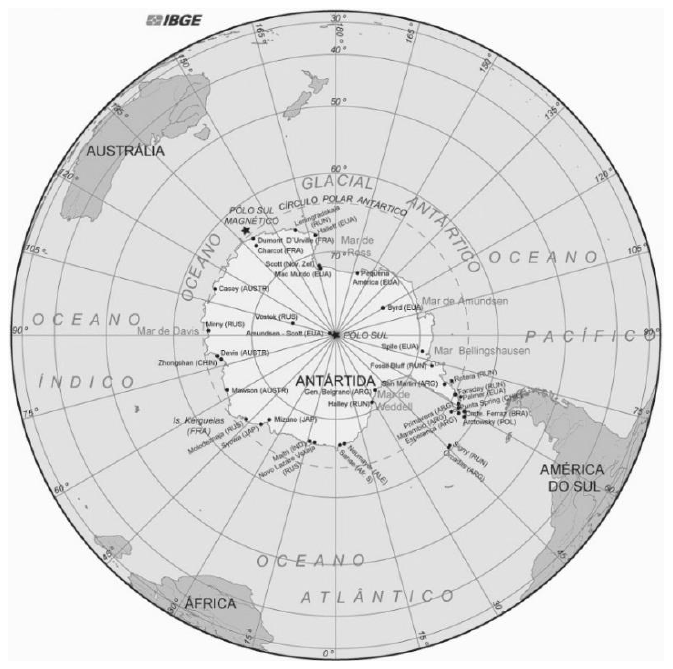
\includegraphics[width=0.95\linewidth]{static/simulados/coluni/figuras/2021/questao-33/figura-1.png}
\end{figure}
% COLUNI-AUTO-FIGURES-END

Mapa da Antártida. Disponível em: https://suportegeografico77.blogspot.com/2017/09/mapa-da-antartida.html. Acesso em: 01 dez. 2020.

\par

Assinale a afirmativa INCORRETA sobre o continente antártico:

\begin{enumerate}
\item A Antártica tem função estratégica, rica em petróleo e outros recursos naturais, é um continente que, por
        convenção internacional, não pertence a nenhum país, constituindo bases de pesquisa para vários estudos.
\item O continente, de clima polar, caracteriza-se por temperaturas extremas, negativas na maior parte do ano,
        o que justifica, entre outros fatores, a presença de grandes geleiras.
\item A Antártica é cobiçada por vários países e, atualmente, alguns deles mantêm bases de pesquisas
        científicas espalhadas pelo continente, demonstrando interesses geopolíticos na região.
\item O continente é o habitat natural de ursos polares e de pinguins, une-se à Terra do Fogo por meio da
        Península Antártica, sendo margeado pelo Oceano Glacial Ártico.\end{enumerate}
